\documentclass[a4paper]{article} 
\usepackage{amsmath,amsfonts,bm}
\usepackage{hyperref}
\usepackage{amsthm} 
\usepackage{geometry}
\usepackage{amssymb}
\usepackage{pstricks-add}
\usepackage{framed,mdframed}
\usepackage{graphicx,color} 
\usepackage{mathrsfs,xcolor} 
\usepackage[all]{xy}
\usepackage{fancybox} 
\usepackage{xeCJK}
\usepackage{pgf,tikz}
\usetikzlibrary{arrows}
\newtheorem{theorem}{定理}
\newtheorem{lemma}{引理}
\newtheorem{corollary}{推论}
\newtheorem*{exercise}{习题}
\newtheorem{example}{例}
\newcommand{\degre}{\ensuremath{^\circ}}
\geometry{left=2.5cm,right=2.5cm,top=2.5cm,bottom=2.5cm}
\setCJKmainfont[BoldFont=Adobe Heiti Std R]{Adobe Song Std L}
\renewcommand{\today}{\number\year 年 \number\month 月 \number\day 日}
\newcommand{\D}{\displaystyle}
\newcommand{\ds}{\displaystyle} \renewcommand{\ni}{\noindent}
\newcommand{\pa}{\partial} \newcommand{\Om}{\Omega}
\newcommand{\om}{\omega} \newcommand{\sik}{\sum_{i=1}^k}
\newcommand{\vov}{\Vert\omega\Vert} \newcommand{\Umy}{U_{\mu_i,y^i}}
\newcommand{\lamns}{\lambda_n^{^{\scriptstyle\sigma}}}
\newcommand{\chiomn}{\chi_{_{\Omega_n}}}
\newcommand{\ullim}{\underline{\lim}} \newcommand{\bsy}{\boldsymbol}
\newcommand{\mvb}{\mathversion{bold}} \newcommand{\la}{\lambda}
\newcommand{\La}{\Lambda} \newcommand{\va}{\varepsilon}
\newcommand{\be}{\beta} \newcommand{\al}{\alpha}
\newcommand{\dis}{\displaystyle} \newcommand{\R}{{\mathbb R}}
\newcommand{\N}{{\mathbb N}} \newcommand{\cF}{{\mathcal F}}
\newcommand{\gB}{{\mathfrak B}} \newcommand{\eps}{\epsilon}
\renewcommand\refname{参考文献}
\begin{document}
\title{\huge{\bf{复数运算的几何意义}}} \author{\small{叶卢
    庆\footnote{叶卢庆(1992---),男,杭州师范大学理学院数学与应用数学专业
      本科在读,E-mail:h5411167@gmail.com}}\\{\small{杭州师范大学理学院,浙
      江~杭州~310036}}}
\maketitle
我们知道,复数 $a+bi$ 和 $c+di$ 的相加定义为
$$
(a+bi)+(c+di)=(a+c)+(b+d)i,
$$
相乘定义为
$$
(a+bi)(c+di)=(ac-bd)+(ad+bc)i.
$$
其中 $i^2=-1$.把 $a+bi$ 和 $c+di$ 分别看作平面直角坐标系上的点 $(a,b)$
和 $(c,d)$.我们先来看复数加法运算的几何意义.如图,\\
\newrgbcolor{xdxdff}{0.49 0.49 1}
\psset{xunit=1.0cm,yunit=1.0cm,algebraic=true,dotstyle=o,dotsize=3pt 0,linewidth=0.8pt,arrowsize=3pt 2,arrowinset=0.25}
\begin{pspicture*}(-8.56,-5.44)(13.47,4.38)
\psaxes[labelFontSize=\scriptstyle,xAxis=true,yAxis=true,Dx=1,Dy=1,ticksize=-2pt 0,subticks=2]{->}(0,0)(-8.56,-5.44)(13.47,4.38)
\rput[tl](1,2.43){$$ (a,b) $$}
\psline{->}(0,0)(1.73,2.1)
\psline{->}(1.73,2.1)(4.64,2.14)
\psline{->}(4.64,2.14)(4.62,-1.67)
\psline{->}(0,0)(3,0)
\psline{->}(3,0)(3,-4)
\psline{->}(0,0)(3,-4)
\psline{->}(1.73,2.1)(4.62,-1.68)
\psline{->}(3,-4)(4.62,-1.68)
\rput[tl](4.9,2.48){$$ (a+c,b) $$}
\rput[tl](4.77,-1.46){$$ (a+c,b+d) $$}
\rput[tl](2.42,0.61){$$ (c,0) $$}
\rput[tl](3.18,-3.83){$$ (c,d) $$}
\begin{scriptsize}
\psdots[dotstyle=*,linecolor=blue](1.73,2.1)
\rput[bl](1.79,2.2){\blue{$A$}}
\psdots[dotstyle=*,linecolor=darkgray](0,0)
\rput[bl](0.07,0.09){\darkgray{$A'$}}
\psdots[dotstyle=*,linecolor=blue](4.64,2.14)
\rput[bl](4.71,2.24){\blue{$B$}}
\psdots[dotstyle=*,linecolor=blue](4.62,-1.68)
\rput[bl](4.69,-1.58){\blue{$C$}}
\psdots[dotstyle=*,linecolor=xdxdff](3,0)
\rput[bl](3.07,0.09){\xdxdff{$B'$}}
\psdots[dotstyle=*,linecolor=blue](3,-4)
\rput[bl](3.07,-3.91){\blue{$C'$}}
\end{scriptsize}
\end{pspicture*}
一图胜千言,我不再说什么了.从上图很容易看出,复数相加的几何意义正是平面
上向量相加的平行四边形法则.下面我们来解释复数相乘的几何意义.\\

我们先看$(a+bi)c$,其中 $c$ 是实数.此时,易得复数 $a+bi$ 与 $c$ 相乘,只
是把点 $(a,b)$ 变成 $(ac,bc)$,这时候的几何意义是显然的.然后我们来看
$(a+bi)di$,此时,是先把点 $(a,b)$ 变成 $(-b,a)$,然后再把点 $(-b,a)$ 变
成 $(-bd,ad)$.综合起来,几何意义如下图:\\
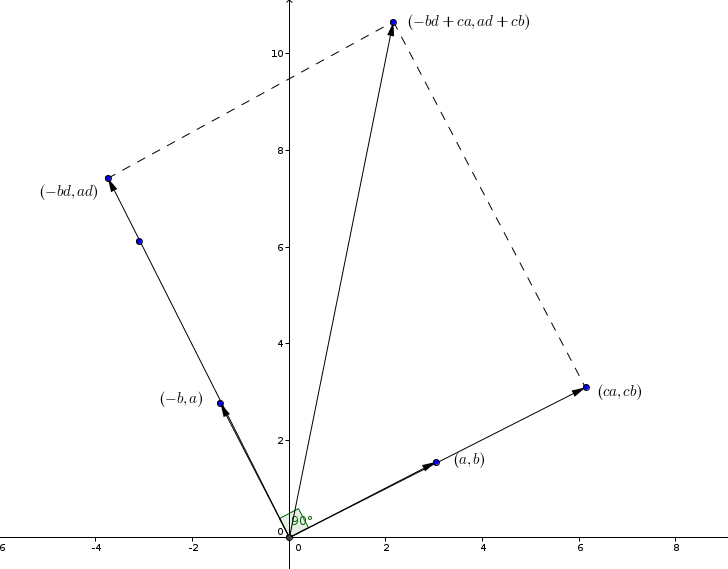
\includegraphics[width=1\textwidth]{/home/luqing/math/visual-complex-analysis/2014-02-23-19-08.png}
\end{document}








